\textbf{5-1} 如力图5-1-1，静止的圆锥体竖直放置，顶角为 $\alpha$。质量为 $m$ 且分布均匀的链条环水平地套在圆锥体上，忽略链条与圆锥体之间的摩擦力。试求链条中的张力。

\begin{center}
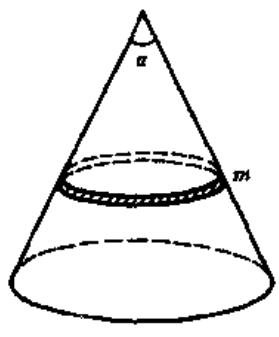
\includegraphics[width=0.15\textwidth]{figures/力图5-1-1.jpg}
\end{center}
\vfill

\textbf{5-2} 如力图5-2-1，均匀杆 $AB$ 长 $l$，重 $w_0$，$A$ 端与粗糙的竖直墙接触，$B$ 端用不可伸长的绳悬挂于竖直墙的 $C$ 点，杆呈水平状态，绳与杆的夹角为 $\theta$。

试问：1. 为了使杆达到静力平衡，杆 A 端与竖直墙之间的摩擦系数 $\mu$ 应满足什么条件？2. 若在杆上悬挂另一重量为 $w = \dfrac{w_0}{2}$ 的重物，为了使杆仍维持平衡，所需摩擦系数的最小值与悬点的位置有何关系？

\begin{center}
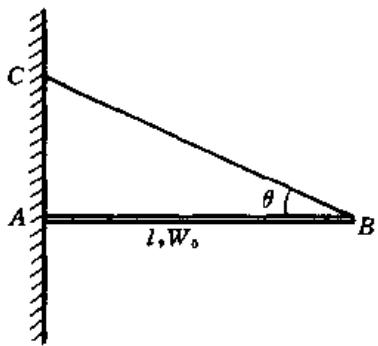
\includegraphics[width=0.2\textwidth]{figures/力图5-2-1.jpg}
\end{center}
\vfill

\newpage
\textbf{5-3} 如力图5-3-1，质量为 $m$、长为 $L$ 的均匀细直杆竖直放置，杆下端与地面之间的摩擦系数为 $\mu$，杆上端用绳索拉住，绳与直杆之间的夹角为 $\theta$。在离地面高度为 $h$ 处以水平力 $F$ 作用于直杆。试问为使直杆不滑倒，作用力 $F$ 的最大值应是多少？

\begin{center}
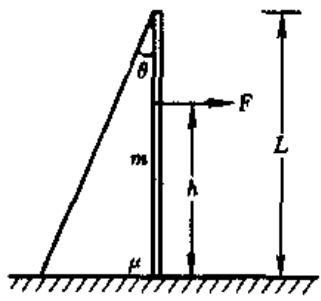
\includegraphics[width=0.2\textwidth]{figures/力图5-3-1.jpg}
\end{center}
\vfill

\textbf{5-4} 如力图5-4-1，在半径为 $R$ 的光滑半球形凹面内，有一刚性均匀细杆达到平衡。已知杆在半球面内那部分的长度为 $l$。试求杆露出半球面外那部分的长度。
\begin{center}
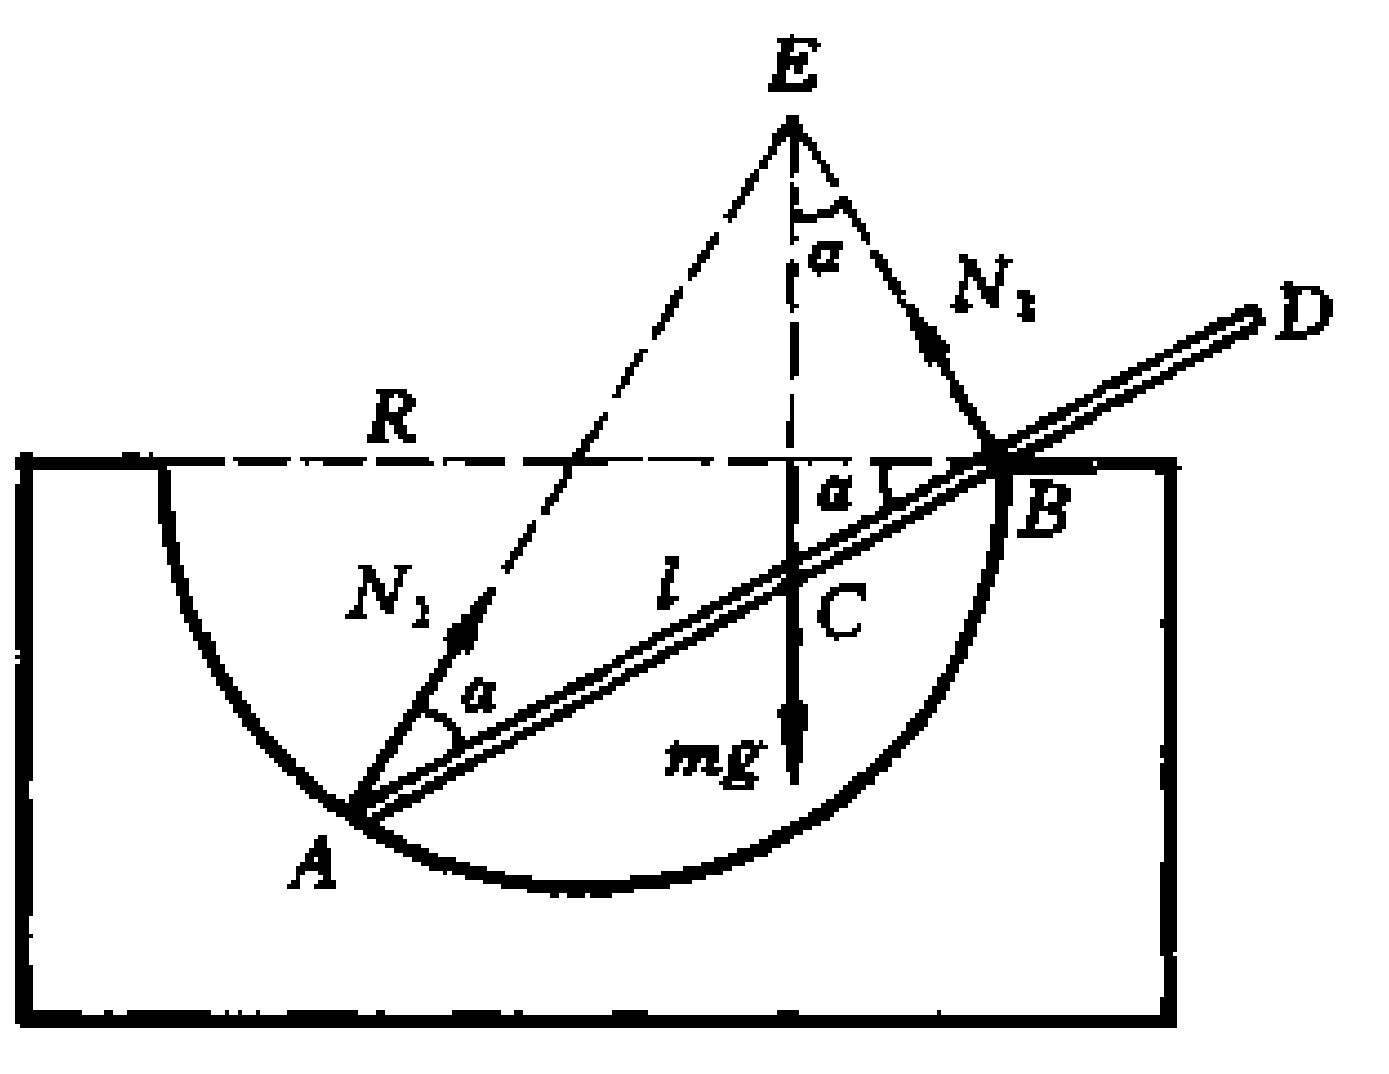
\includegraphics[width=0.2\textwidth]{figures/力图5-4-1.jpg}
\end{center}
\vfill

\newpage
\textbf{5-5} 如力图5-5-1，三个半径和质量均相同的圆柱体按图中的方式堆放在地面上，互相接触。已知圆柱体之间的摩擦系数为 $\mu_{1}$，圆柱体与地面之间的摩擦系数为 $\mu_{2}$。试求使三圆柱体达到平衡所需之 $\mu_{1}$ 和 $\mu_{2}$ 的下限值。

\begin{center}
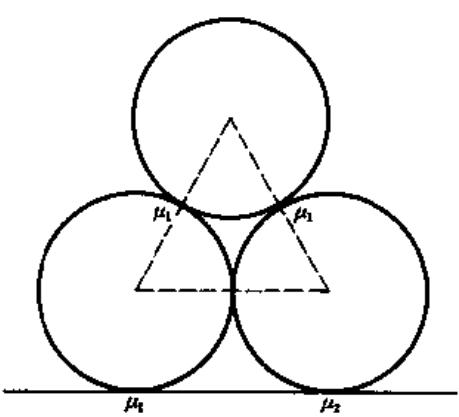
\includegraphics[width=0.2\textwidth]{figures/力图5-5-1.jpg}
\end{center}
\vfill

\textbf{5-6} 如力图5-6-1所示，均匀木板 $AB$ 长 $L = 100\,\mathrm{cm}$，重 $2G$，一端用铰链固定于竖直墙，另一端用水平线拉住，木板与竖直墙之间的夹角为 $60^{\circ}$。三个完全相同的球按力图5-6-1中的位置放在木板上，球半径均为 $R = 10\,\mathrm{cm}$，重量均为 $G$。设球与墙，球与木板，球与球之间的摩擦力均可忽略。试求水平线的拉力 $T$。

\begin{center}
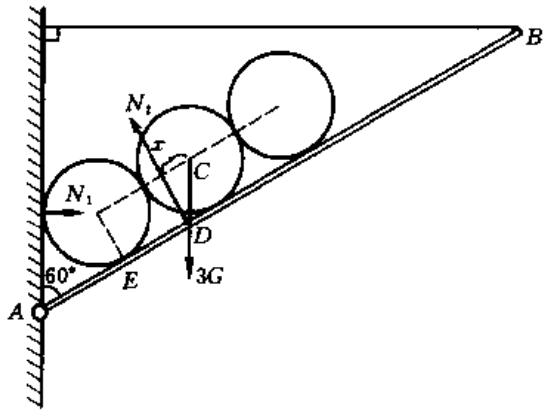
\includegraphics[width=0.3\textwidth]{figures/力图5-6-1.jpg}
\end{center}
\vfill

\newpage
\textbf{5-7} 如力图5-7-1所示，AB、BC、CD和DE为质量可略的等长细线，长度均为 $5\,\mathrm{m}$，$A$ 端和 $E$ 端悬挂在水平天花板上，$AE = 14\,\mathrm{m}$。B 和 D 是质量均为 $m_0 = 7\,\mathrm{kg}$ 的相同小球。质量为 $m$ 的重物挂于 $C$ 点，平衡时 $C$ 点离天花板的垂直距离为 $7\,\mathrm{m}$。

1. 试求质量 $m$。2. 今用外力将 $C$ 点缓慢提升，使BCD位于同一水平线上，试求此过程中外力作的功。

\begin{center}
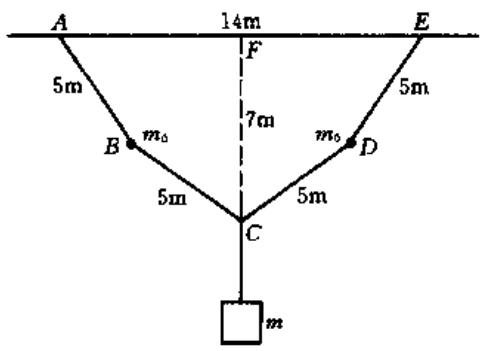
\includegraphics[width=0.2\textwidth]{figures/力图5-7-1.jpg}
\end{center}
\vfill

\textbf{5-8} 如力图5-8-1所示，浮子由两个半径为 $R$ 的球冠相合而成，其质量为 $m_{1}$，中心厚度为 $h$ $(h < 2R)$。长为 $l$，质量为 $m_{2}$ 的均匀细杆从浮子中心垂直插入，下端刚好到达下球冠表面。细杆的铅垂位置显然是一个平衡位置。试分析平衡的稳定性。

\begin{center}
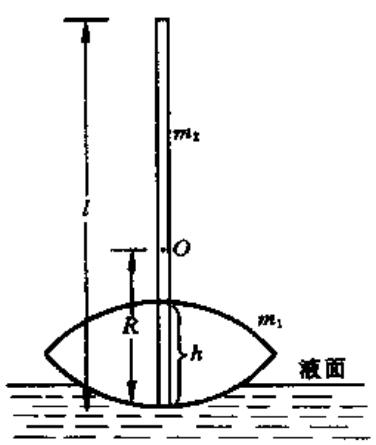
\includegraphics[width=0.2\textwidth]{figures/力图5-8-1.jpg}
\end{center}
\vfill

\newpage
\textbf{5-9} 如力图5-9-1，五根质量分布均匀、质量和长度完全相同的细杆，用光滑铰链互相连结并悬挂起来。试求平衡时由细杆组成的五边形的五个顶角。

\begin{center}
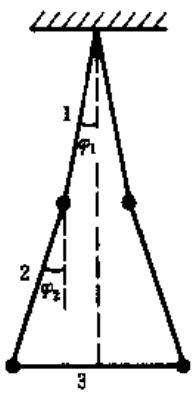
\includegraphics[width=0.12\textwidth]{figures/力图5-9-1.jpg}
\end{center}
\vfill

\textbf{5-10} 如力图5-10-1，半径为 $R$ 的圆柱体在水平面上固定不动，厚度为 $t$ 的均匀木板水平地放置在圆柱体上，其长度方向（力图5-10-1中的横向）与圆柱体的轴（水平方向与力图5-10-1的平面垂直）垂直，并处于平衡状态。试问厚度 $t$ 取何值时属稳定平衡。

\begin{center}
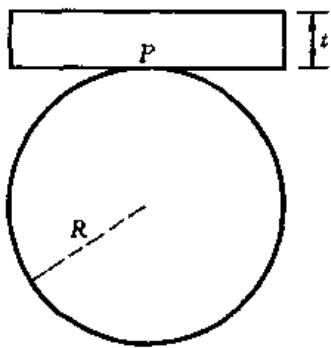
\includegraphics[width=0.2\textwidth]{figures/力图5-10-1.jpg}
\end{center}
\vfill

\newpage
\textbf{5-11} 如力图5-11-1，四根质量、长度都相同的均匀木条用光滑铰链连接成菱形，一均匀圆盘静止地夹在两木条之间，整个系统竖直悬挂起来，悬点为 $O$ 点。设圆盘与木条之间的接触是光滑的。已知每根木条的长度 $l = 50\,\mathrm{cm}$，质量 $m = 50\,\mathrm{g}$；圆盘的半径 $r = 8\,\mathrm{cm}$，质量 $M = 200\,\mathrm{g}$。试求系统的平衡位置（用 $\theta$ 角表示）。
\begin{center}
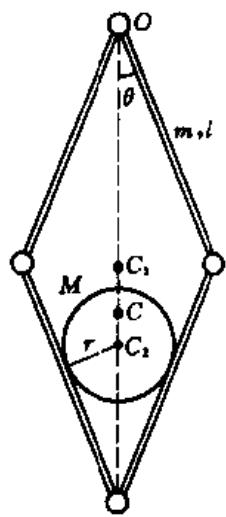
\includegraphics[width=0.1\textwidth]{figures/力图5-11-1.jpg}
\end{center}
\vfill

\textbf{5-12} 如力图5-12-1，质量分布均匀的柔软细绳全长 $L$，质量线密度为 $\lambda$，悬挂在两根竖直杆上，测得细绳在两悬挂点的切线与竖直杆之间的夹角分别为 $\theta_{1}$ 和 $\theta_{2}$。

1. 试求细绳两端所受的拉力。2. 若左悬点的高度为 $H$，试导出在 $Oxy$ 坐标系中的悬链线方程。

\begin{center}
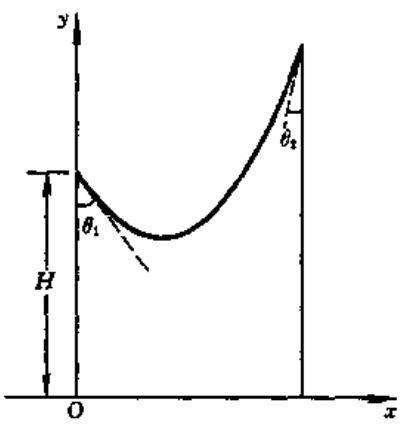
\includegraphics[width=0.18\textwidth]{figures/力图5-12-1.jpg}
\end{center}
\vfill

